\documentclass{article}

\usepackage{graphicx}
\usepackage[margin=0.5in]{geometry}
\usepackage{amsmath}
\usepackage{amssymb}
\usepackage[T1]{fontenc}
\usepackage{listings}
\usepackage{psfrag}
\usepackage{alltt}
\usepackage{rotating}
\usepackage{color}

\pagenumbering{gobble}


\begin{document}

%
%
%

%
\section{Rosebrock}
%
\begin{figure}[h!]
        \begin{center}
                \begin{minipage}[h!]{0.32\textwidth}
                        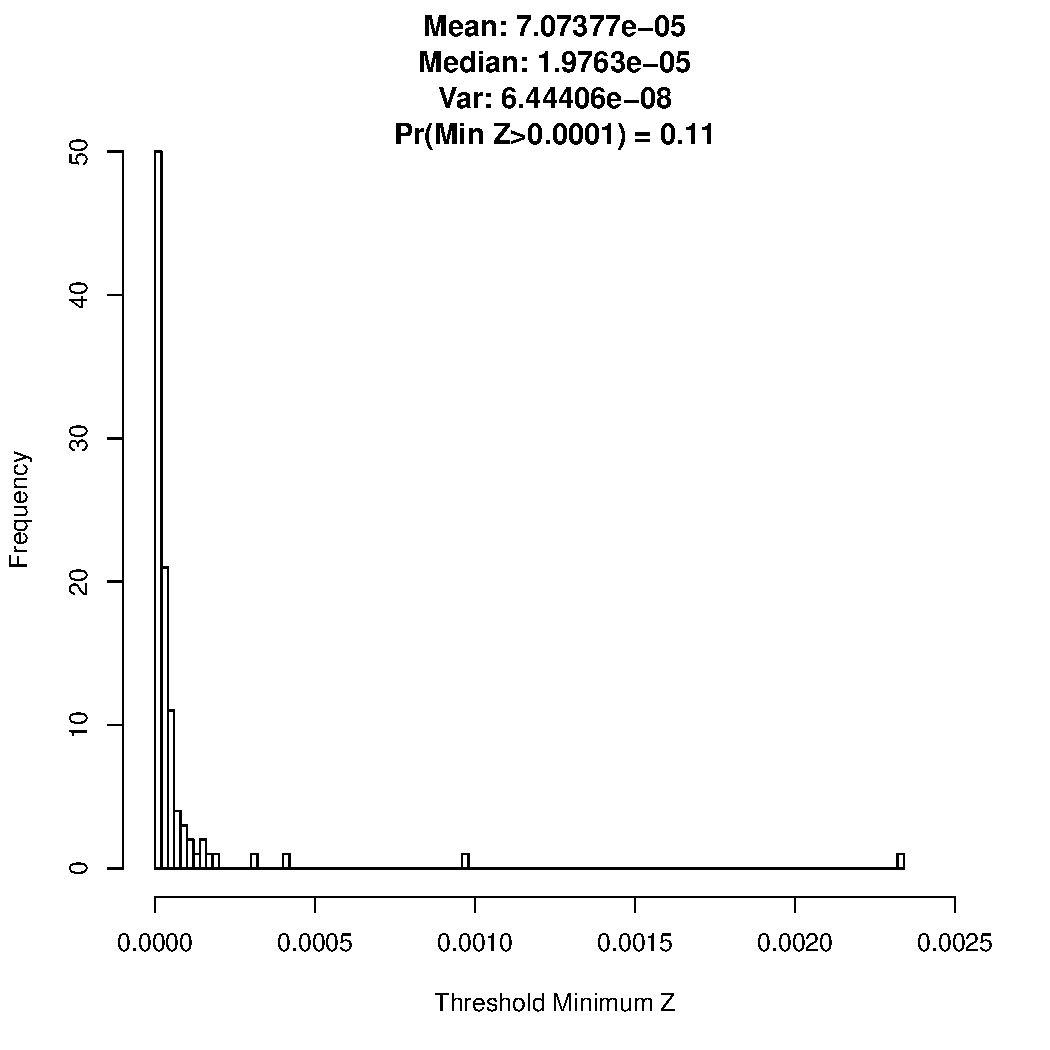
\includegraphics[width=1.0\textwidth]{threshSimHist.pdf}
                \end{minipage}
                \begin{minipage}[h!]{0.32\textwidth}
                        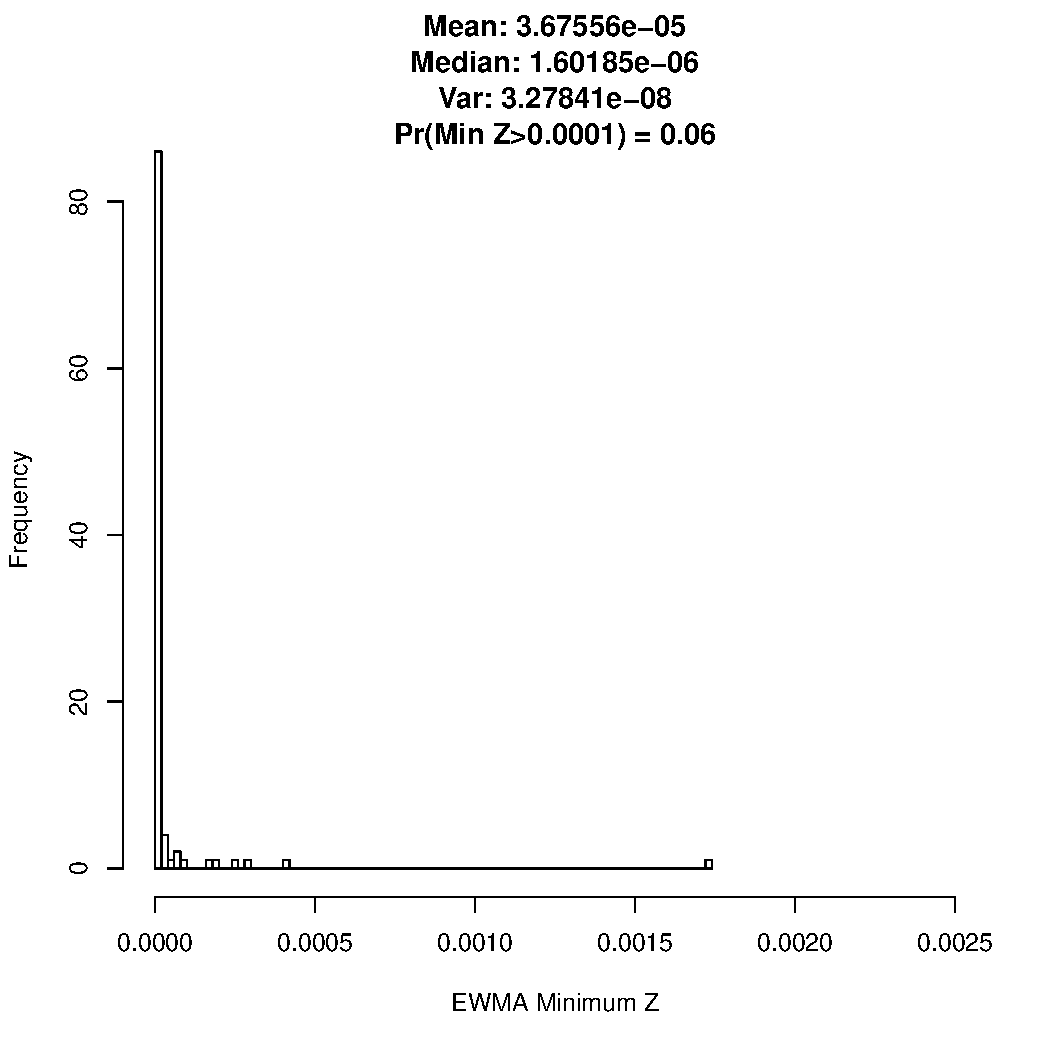
\includegraphics[width=1.0\textwidth]{ewmaSimHist.pdf}
                \end{minipage}
		\begin{minipage}[h!]{0.32\textwidth}
                        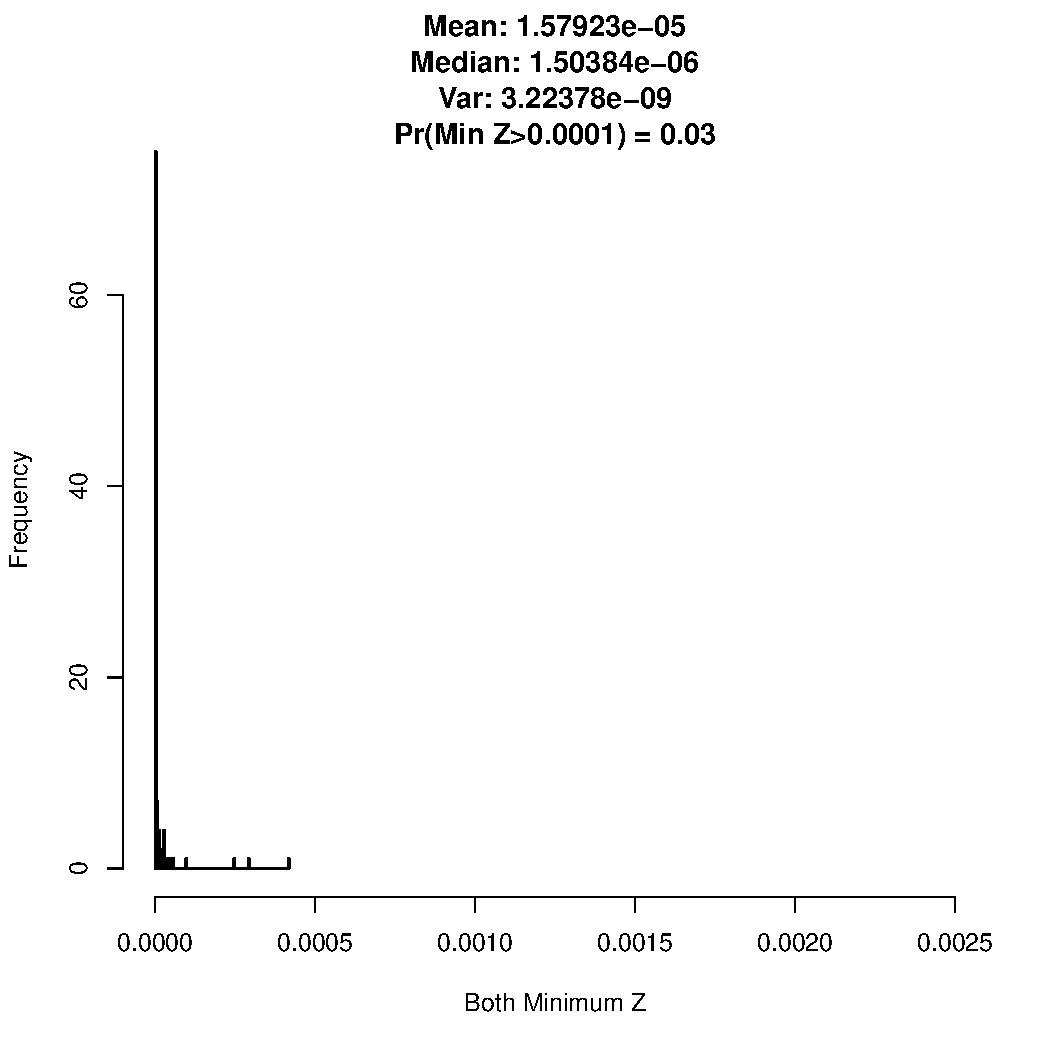
\includegraphics[width=1.0\textwidth]{bothSimHist.pdf}
                \end{minipage}
        \end{center}
\end{figure}

%
%
%

\section{\color{red}Rastrigin}

%
\begin{figure}[h!]
        \begin{center}
                \begin{minipage}[h!]{0.32\textwidth}
                        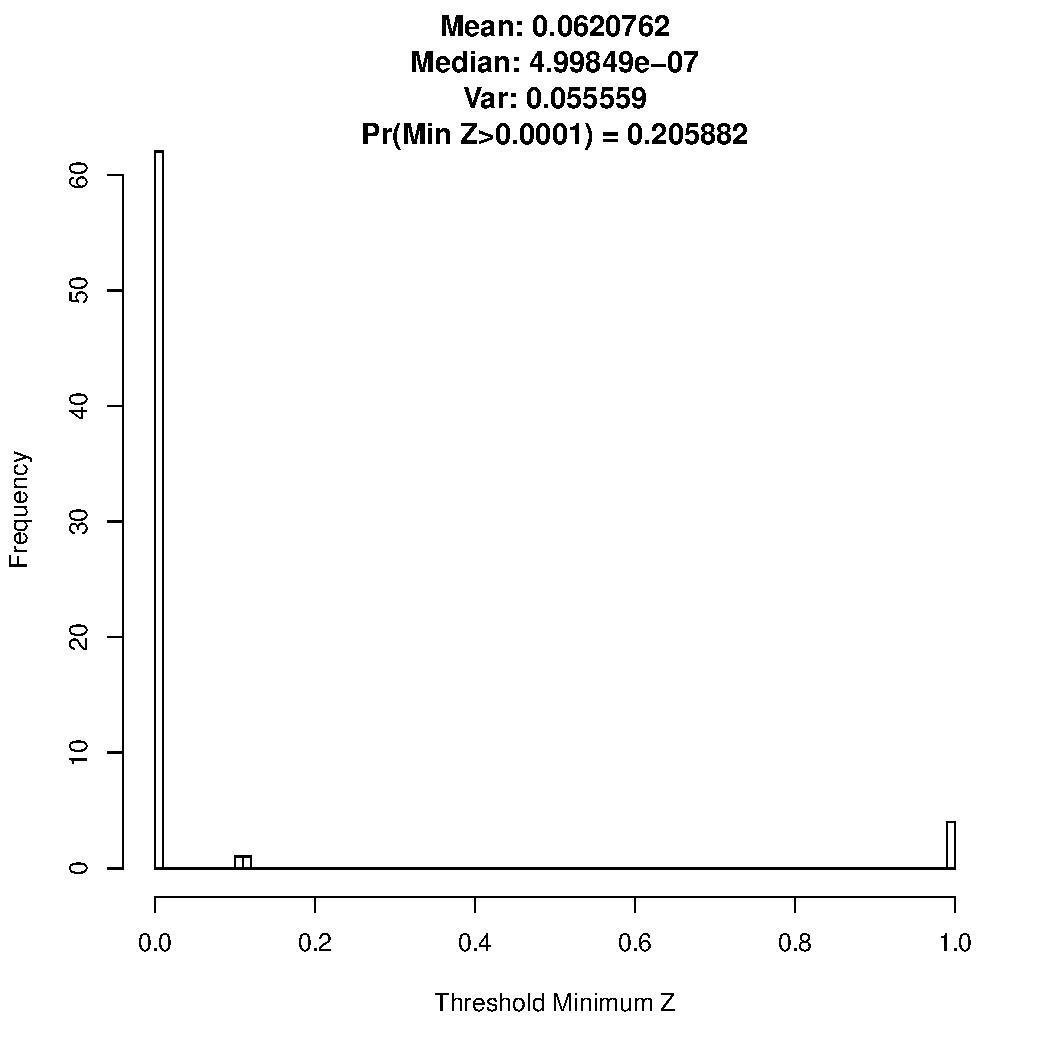
\includegraphics[width=1.0\textwidth]{threshSimHistRast.pdf}
                \end{minipage}
                \begin{minipage}[h!]{0.32\textwidth}
                        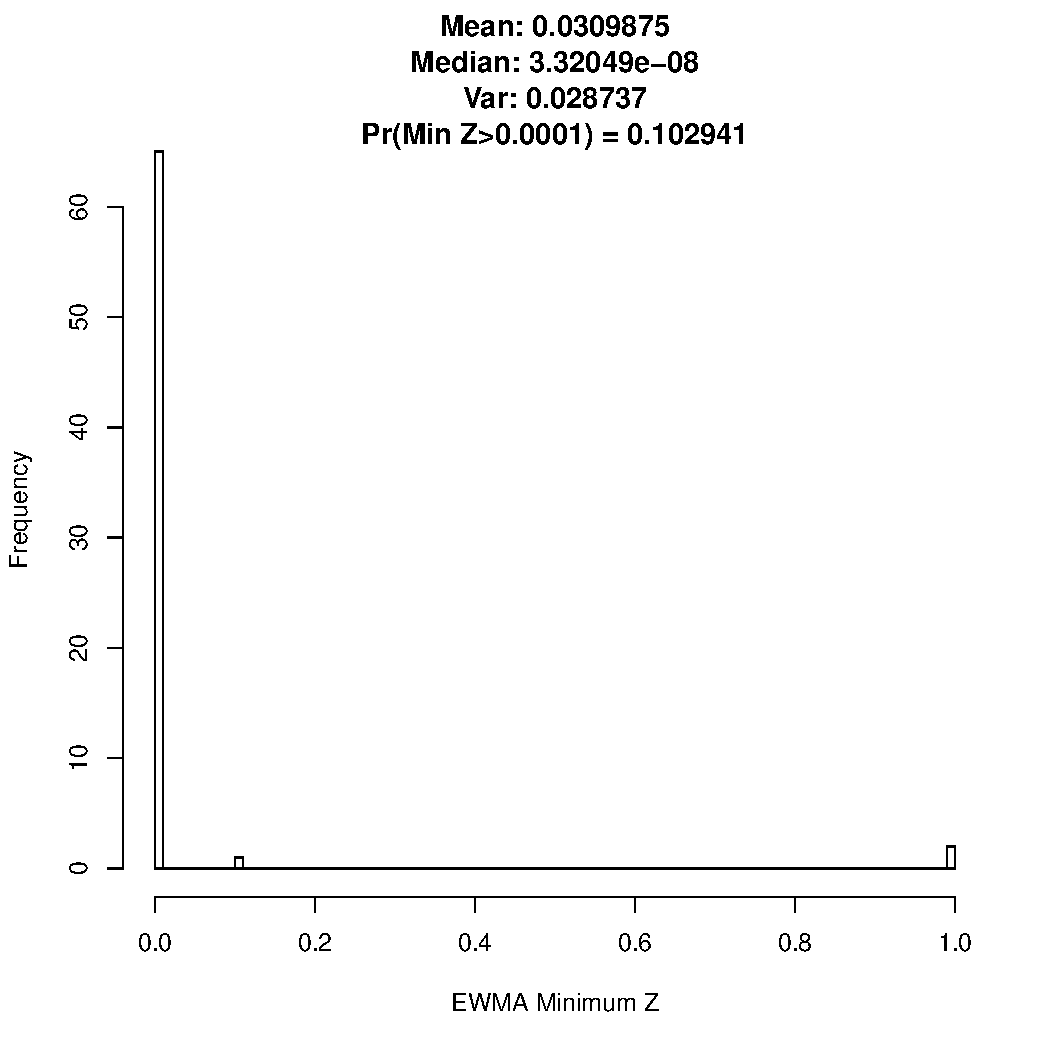
\includegraphics[width=1.0\textwidth]{ewmaSimHistRast.pdf}
                \end{minipage}
		\begin{minipage}[h!]{0.32\textwidth}
                        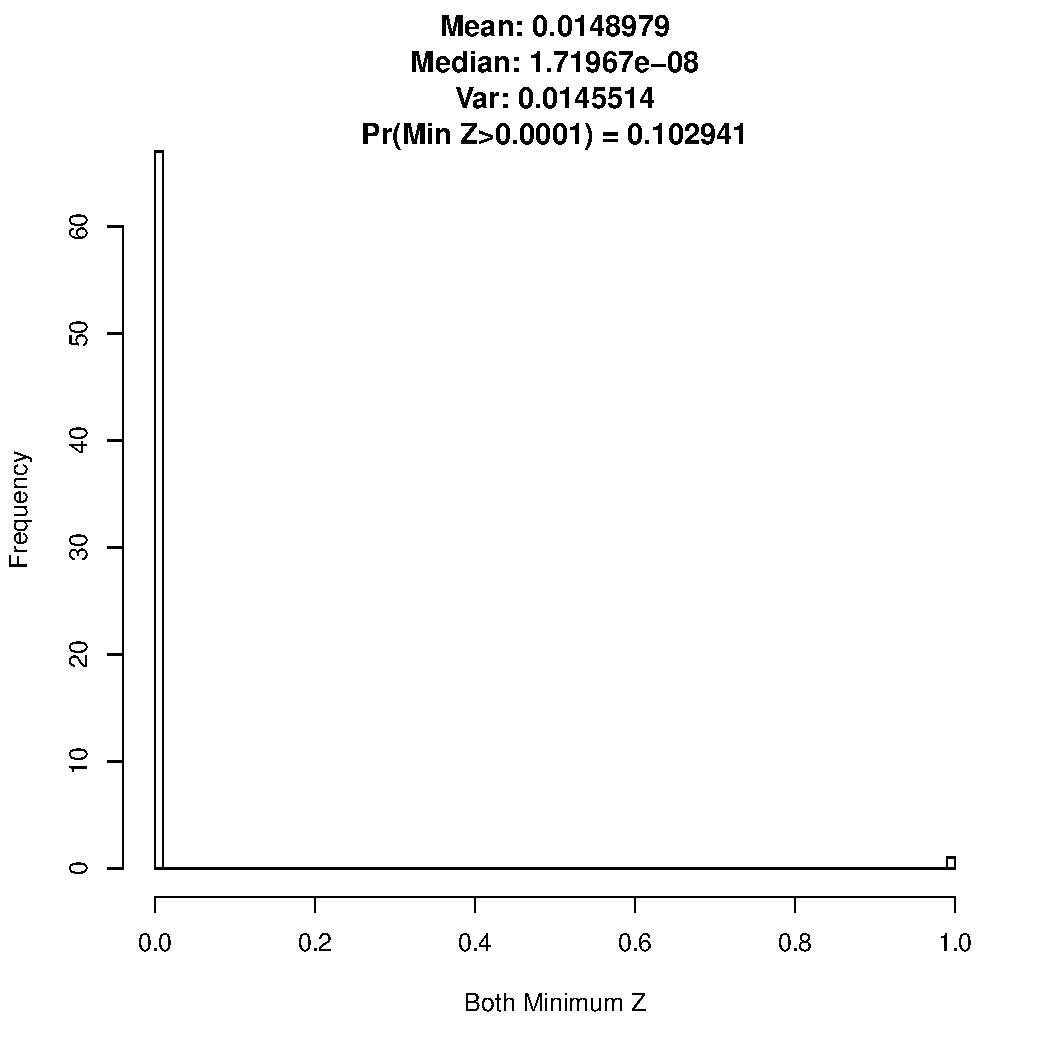
\includegraphics[width=1.0\textwidth]{bothSimHistRast.pdf}
                \end{minipage}
		
        \end{center}
\end{figure}

%
%
%

%
\section{\color{red}Iterations Until Stop}
%
\begin{figure}[h!]
	\begin{center}
	\begin{minipage}[h!]{0.32\textwidth}
		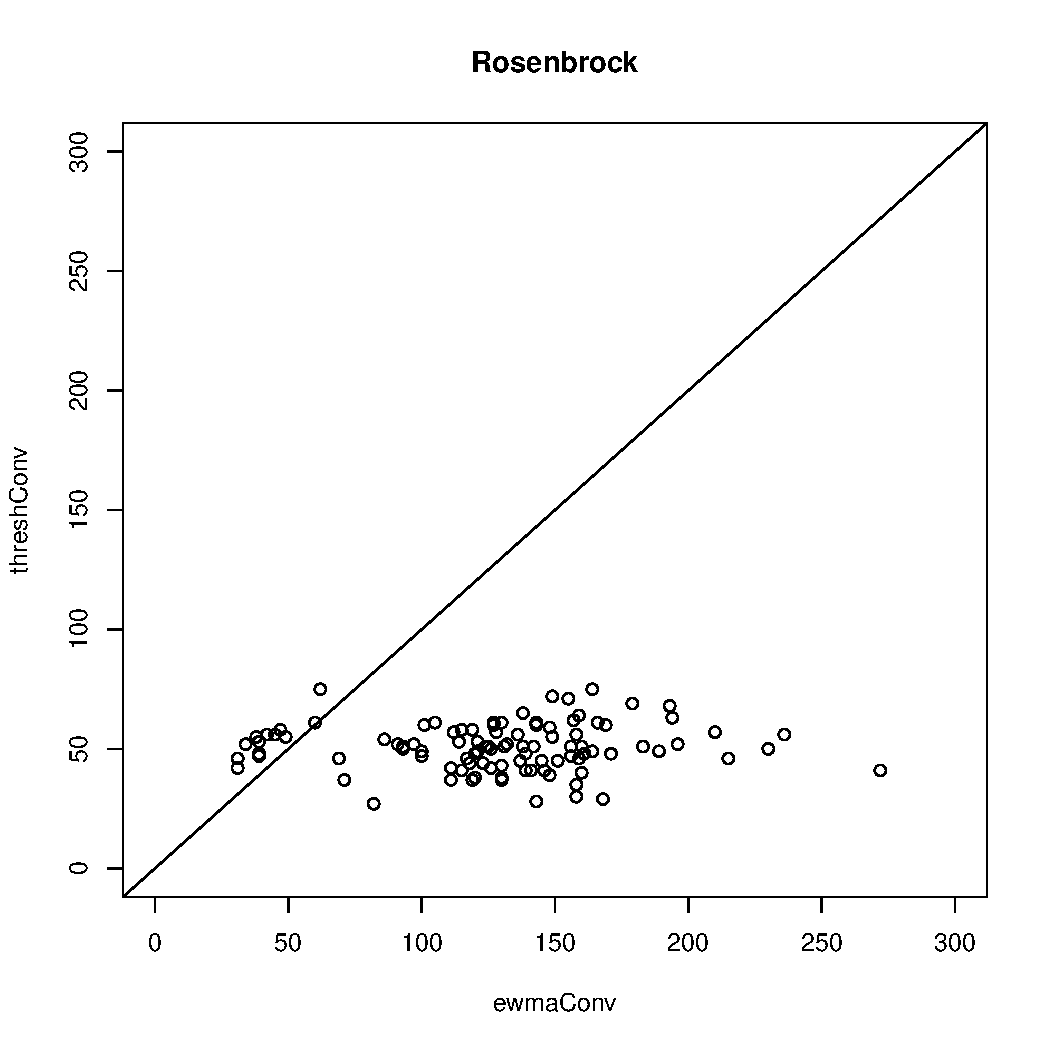
\includegraphics[width=1\textwidth]{itConv.pdf}
	\end{minipage}
	\begin{minipage}[h!]{0.32\textwidth}
		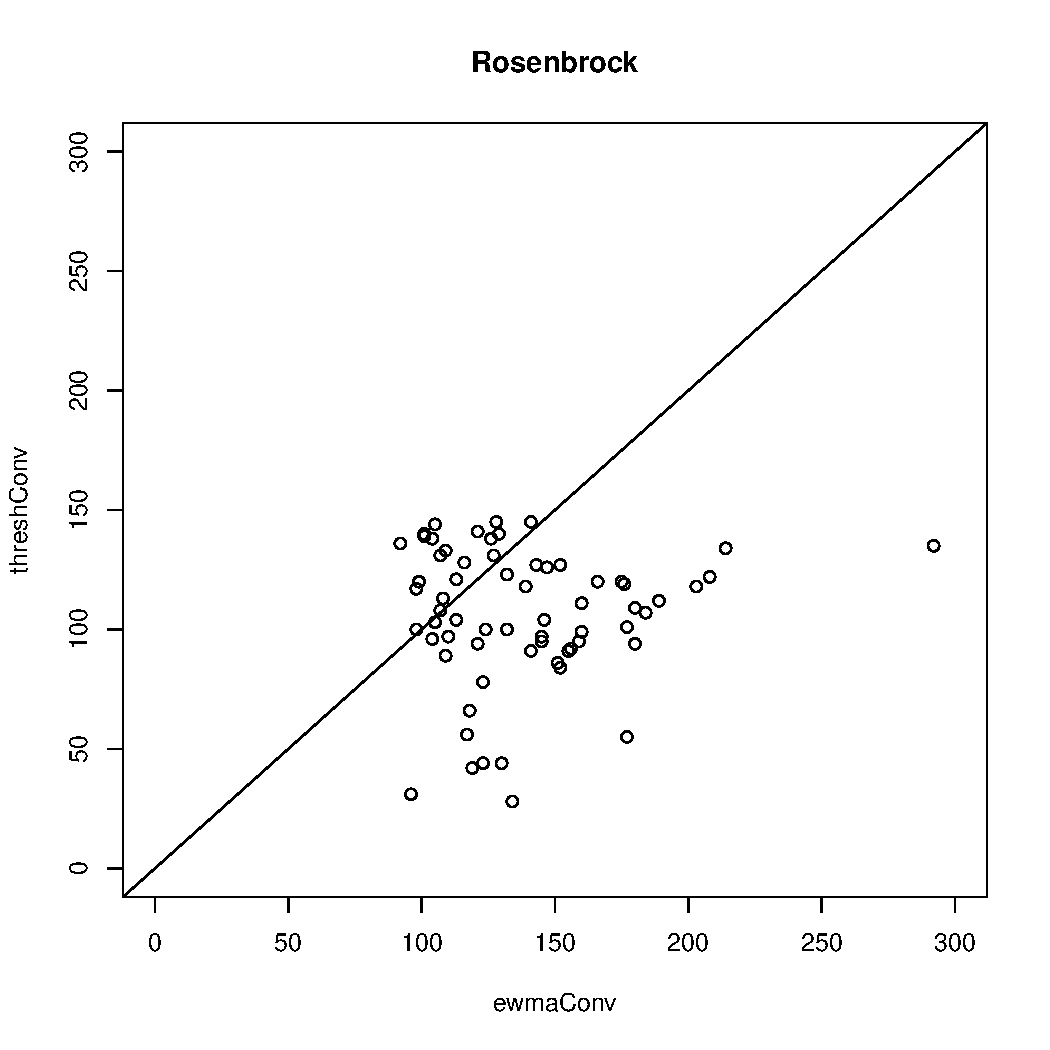
\includegraphics[width=1\textwidth]{itConvRast.pdf}
	\end{minipage}
	\end{center}
\end{figure}

%
%
%

%
\section{Thoughts}
%
\begin{itemize}
\item I think the choice of $w$ just depends on the observed variance in the convergence metric.
	\begin{itemize}
		\item observed variance will be a function of dimension
		\begin{itemize}
			\item Could imagine finding some approxiate function via large simulation over many different objective types
		\end{itemize}
		\item adaptive $w$ dependent on the observed variance?
	\end{itemize}
\end{itemize}

%
%
%

%
\section{Writting Goals}
%
\begin{itemize}
\item
\end{itemize}






%\begin{sidewaysfigure}[h!]
%        \begin{center}
%                \begin{minipage}[h!]{0.49\textwidth}
%                        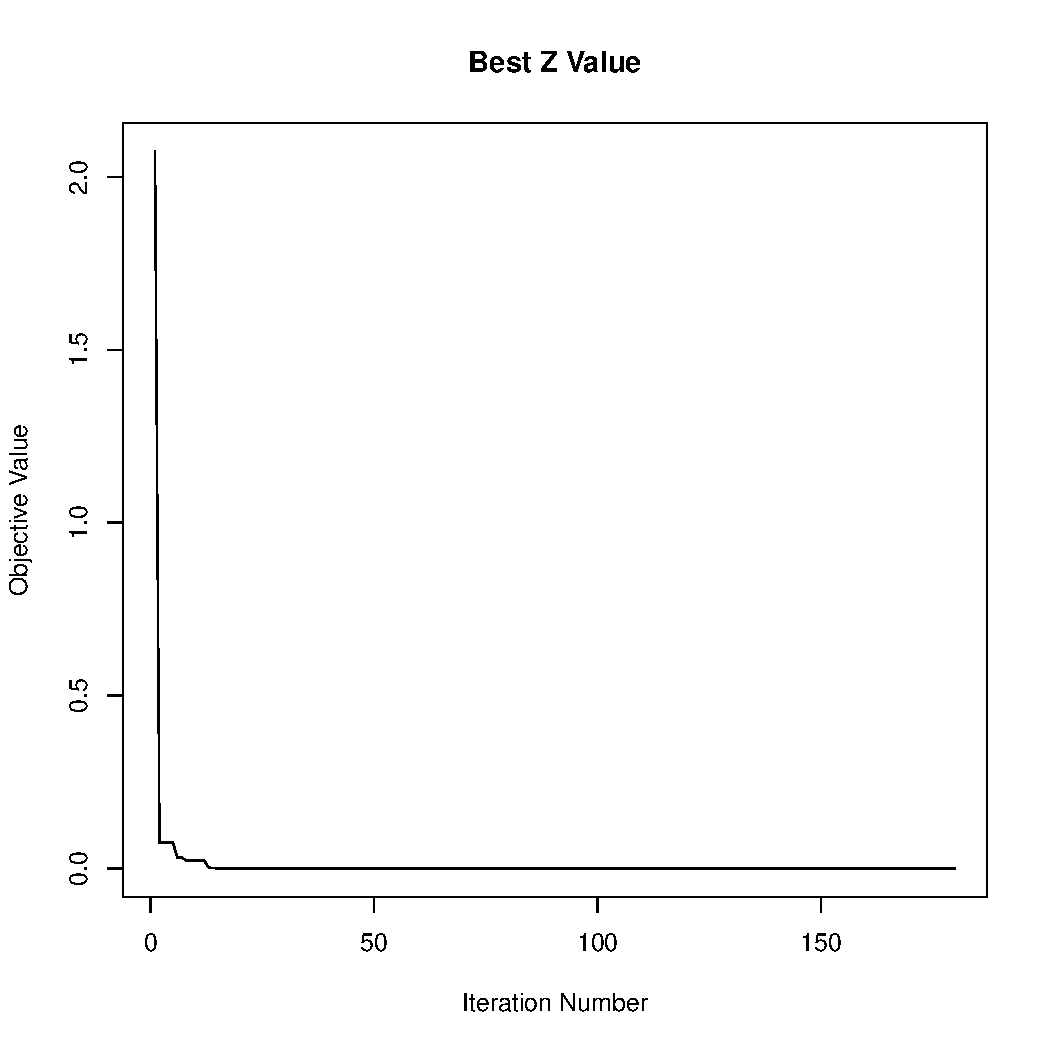
\includegraphics[width=1.0\textwidth]{pictures/bestZrosenbrockThirtyMPI999.pdf}
%                \end{minipage}
%                \begin{minipage}[h!]{0.49\textwidth}
%                        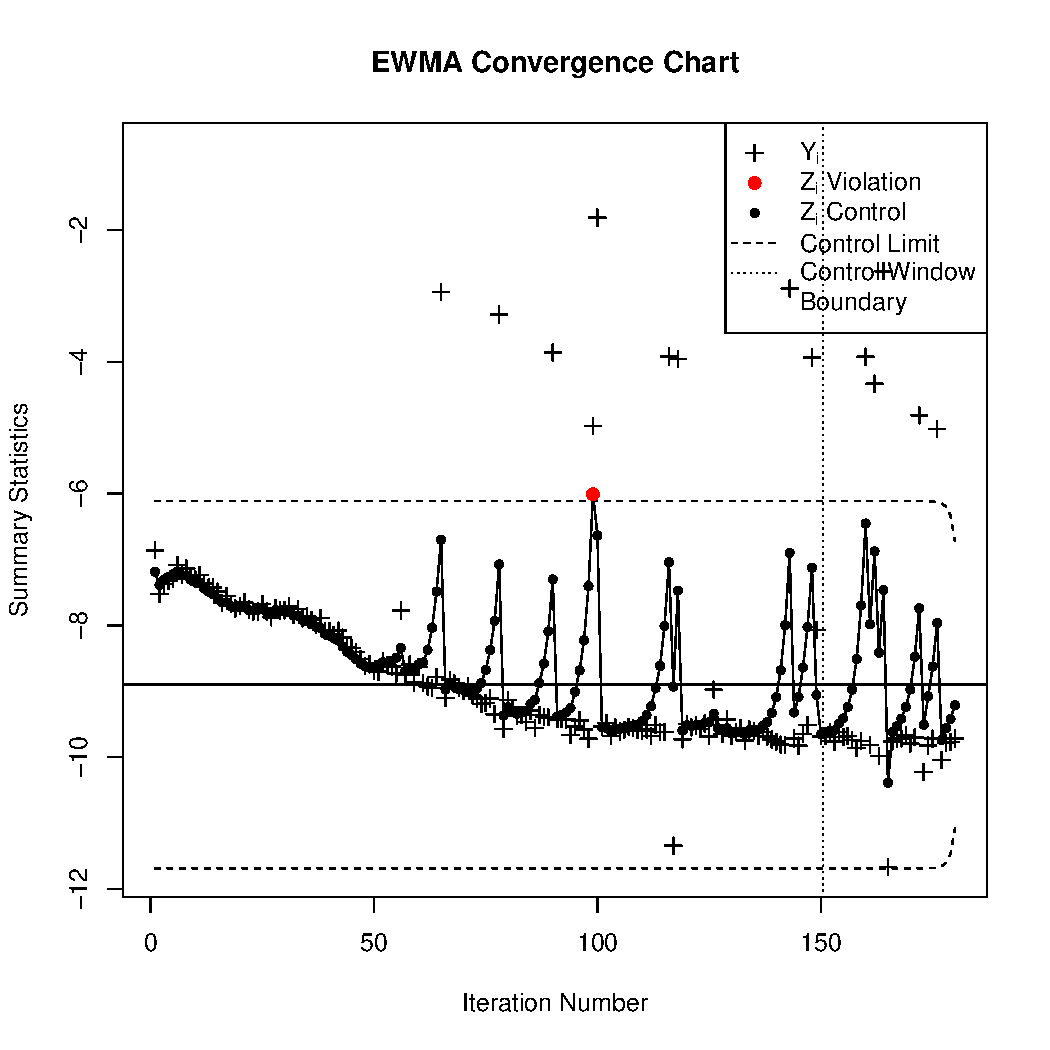
\includegraphics[width=1.0\textwidth]{pictures/ewmaConvChartrosenbrockThirtyMPI999.pdf}
%                \end{minipage}
%        \end{center}
%\end{sidewaysfigure}

\clearpage

\end{document}

